\documentclass[
	12pt,
	a4paper,
	article,
	twocolumn,
	brazil
]{abntex2}

% --- Pacotes Básicos do AbnTeX2 ---
\usepackage{lmodern}
\usepackage[T1]{fontenc}
\usepackage[utf8]{inputenc}
\usepackage{indentfirst}
\usepackage{graphicx}
\graphicspath{{figuras/}{./}}
\usepackage{amsmath,amssymb}
\usepackage{booktabs}
\usepackage{hyperref}

\hypersetup{
	colorlinks=true,
	linkcolor=blue,
	citecolor=blue,
	urlcolor=blue
}

% Remove o título em língua estrangeira padrão do abntex2 article
\renewcommand{\maketitlehookb}{}

\titulo{Mini-projeto 1: buscas clássicas e otimização}

\autor{
	Eduardo N. S. R.\\[0.2em]
	\small PPGCO / PGC112 -- Faculdade de Computação (FACOM)\\
	\small Repositório Github: \href{https://github.com/vndmtrx/ppgco-pgc112-ia}{\texttt{vndmtrx/ppgco-pgc112-ia}}
}

\data{Uberlândia -- MG, Brasil, 2026}

\begin{document}
\frenchspacing
\SingleSpacing

\maketitle

\section{Introdução}

Este relatório apresenta a resolução do Mini-Projeto 1 sob duas abordagens da Inteligência Artificial: (i) busca clássica no espaço de estados discreto (BFS e Algoritmo Guloso) e (ii) otimização contínua no hipercubo fuzzy via Gradiente Descendente com regularização por custo de vizinhança.

O problema consiste em transformar a fita inicial canônica de $L = 23$ bits:
\begin{equation}
s_0 = \texttt{00001001000011001100111}
\end{equation}
na fita alvo composta exclusivamente por zeros:
\begin{equation}
s_{\text{alvo}} = \texttt{00000000000000000000000}
\end{equation}

O modelo de custos estabelece que: (i) o flip de 1 bit possui custo unitário 1; e (ii) o flip de um bloco de $n$ bits consecutivos possui custo uniforme 1. Essa regra confere uma economia de escala crítica, na qual inverter agrupamentos adjacentes custa o mesmo que uma modificação isolada.

O código-fonte, a suíte de testes e os benchmarks estão na pasta \textit{mini\_projeto\_1} dentro do repositório Git \href{https://github.com/vndmtrx/ppgco-pgc112-ia}{\texttt{vndmtrx/ppgco-pgc112-ia}}, cujo \texttt{README.md} detalha a instalação e execução em ambiente isolado (\textit{virtualenv}).

\section{Parte I: Buscas Clássicas}

\subsection{Subrotinas para Flips e Álgebra Bitwise}

Para eliminar a sobrecarga de memória do CPython associada à instanciação de strings e objetos no heap durante a geração de milhões de estados, a fita foi representada diretamente como um número inteiro nativo (\texttt{int}). 

As operações de inversão foram executadas diretamente via máscaras binárias com XOR ($\oplus$):
\begin{itemize}
    \item \textbf{Flip de 1 bit:} $\text{estado} \oplus (1 \ll \text{pos})$, para $0 \le \text{pos} < L$.
    \item \textbf{Flip de bloco contíguo:} $\text{estado} \oplus (((1 \ll n) - 1) \ll \text{pos})$, para $2 \le n \le L - \text{pos}$.
\end{itemize}
Adotou-se a ordenação \textit{little-endian} (bit 0 como o menos significativo, $2^0$). Essa representação viabiliza verificar estados visitados com hash $O(1)$ e executar centenas de milhares de flips por segundo.

\subsection{Algoritmo BFS e Solução Ótima}

Como todas as transições possuem custo uniforme unitário ($c = 1$), a primeira solução gerada pela Busca em Largura (BFS) possui garantia formal de otimalidade. O algoritmo foi implementado com fila FIFO (\texttt{deque}) e conjunto de visitados (\texttt{set}), realizando o teste de objetivo antecipado na geração do nó.

Para a sequência canônica de 23 bits, o algoritmo retornou o \textbf{custo ótimo igual a 5} e a seguinte sequência de operações:
\begin{equation*}
\begin{aligned}
\mathcal{S}_{\text{BFS}} = [ & (\texttt{'bit'}, 15), (\texttt{'bit'}, 18), \\
& (\texttt{'bloco'}, 3, 2), (\texttt{'bloco'}, 7, 2), \\
& (\texttt{'bloco'}, 0, 11) ]
\end{aligned}
\end{equation*}
onde $(\texttt{'bloco'}, \text{pos}, n)$ inverte $n$ bits consecutivos a partir de $\text{pos}$, e $(\texttt{'bit'}, \text{pos})$ inverte a coordenada individual. Para alcançar essa profundidade $d = 5$, o BFS expandiu \textbf{752.059 nós}, visitou \textbf{2.745.489 estados} e consumiu \textbf{35,42 s}. O comportamento de crescimento de nós do algoritmo é ilustrado na Figura~\ref{fig:bfs_nos}.

\begin{figure}[htbp]
\centering
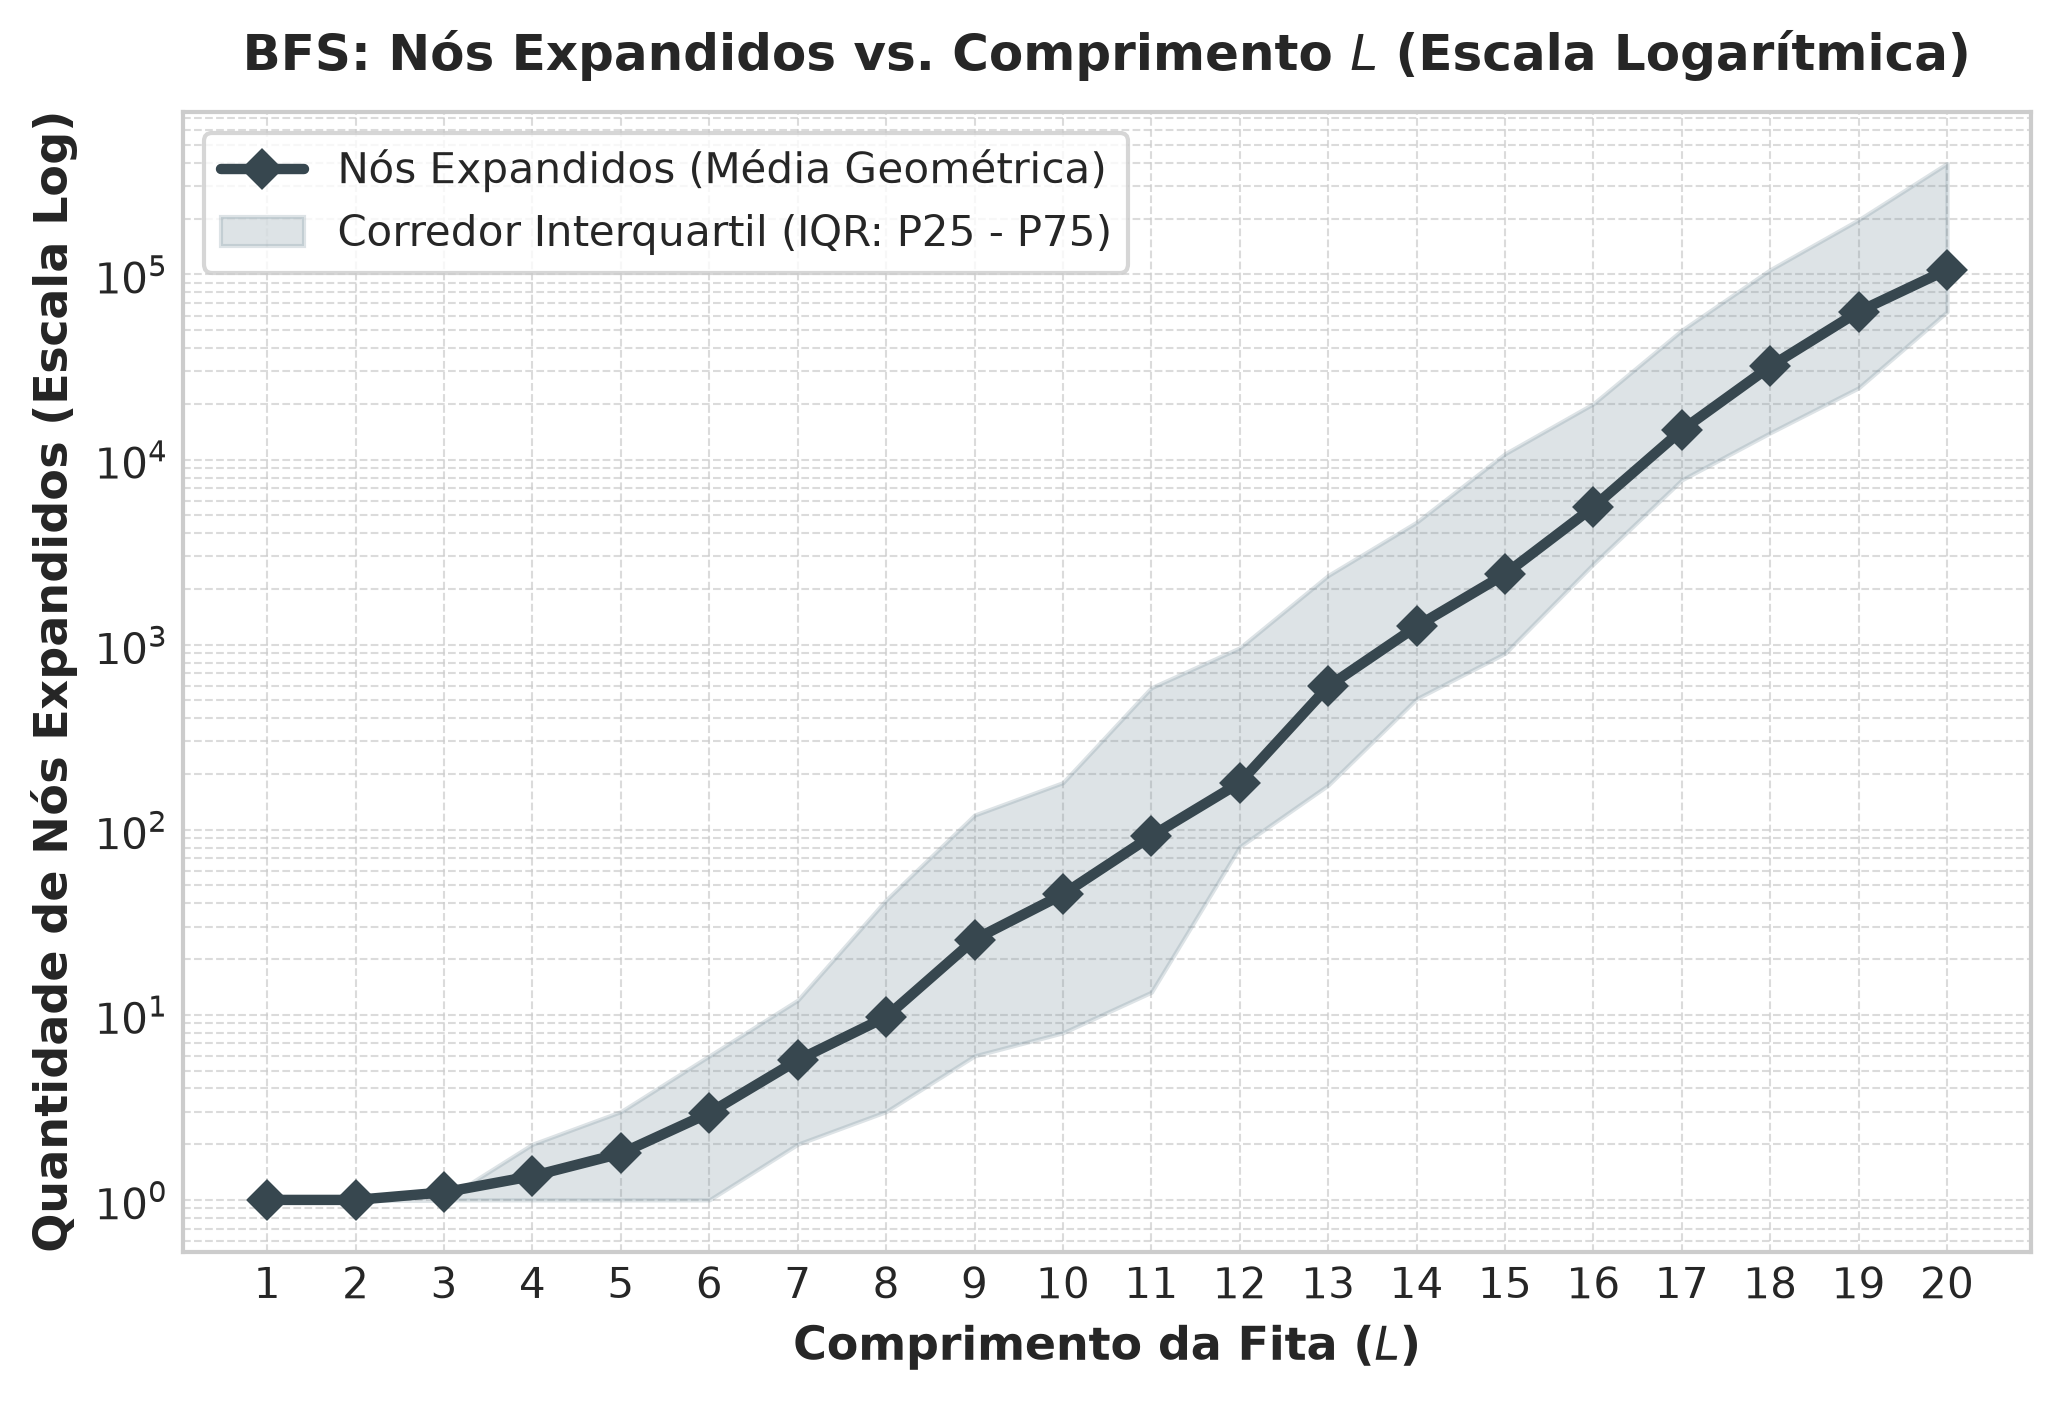
\includegraphics[width=\columnwidth]{grafico_bfs_nos_expandidos.png}
\caption{Crescimento exponencial do número de nós expandidos pelo BFS em função de $L$ no pior caso teórico.}
\label{fig:bfs_nos}
\end{figure}

\subsection{Algoritmo Guloso e Heurísticas}

A Busca Gulosa de Melhor Escolha utiliza uma função heurística $h(s)$ para priorizar estados com menor custo estimado até o alvo:
\begin{itemize}[nosep]
    \item \textbf{Distância de Hamming ($h_1$):} Conta o número absoluto de bits 1 ($h_1(s_0) = 9$). Como flips de bloco eliminam múltiplos 1s sob custo unitário, $h_1$ superestima o custo real ($9 > 5$), violando a admissibilidade ($h(s) \le h^*(s)$).
    \item \textbf{Contagem de Blocos Contíguos ($h_2$):} Avalia quantos agrupamentos contíguos de 1s existem na fita ($h_2(s_0) = 5$). Como cada bloco conexo pode ser extinto em uma única operação de custo 1, $h_2$ coincide com o custo real ótimo ($h_2(s) = h^*(s)$), garantindo monotonicidade estrita.
\end{itemize}

\paragraph{Poda de Ciclos.} Devido à miopia do Guloso, sem memória histórica o algoritmo pode alternar flips reversíveis e entrar em \textbf{loops infinitos}. Com a inclusão da tabela hash de visitados (\textit{poda de ciclos}), a busca gulosa com $h_2$ retornou o \textbf{custo total igual a 5} e a sequência de transformações:
\begin{equation*}
\begin{aligned}
\mathcal{S}_{\text{Guloso}} = [ & (\texttt{'bloco'}, 0, 3), (\texttt{'bloco'}, 5, 2), \\
& (\texttt{'bloco'}, 9, 2), (\texttt{'bit'}, 15), \\
& (\texttt{'bit'}, 18) ]
\end{aligned}
\end{equation*}
atingindo o alvo ótimo em exatamente \textbf{5 expansões} e tempo de \textbf{0,16 ms}. A Figura~\ref{fig:guloso_poda} ilustra a eficácia da poda na contenção do tempo de processamento.

\begin{figure}[htbp]
\centering
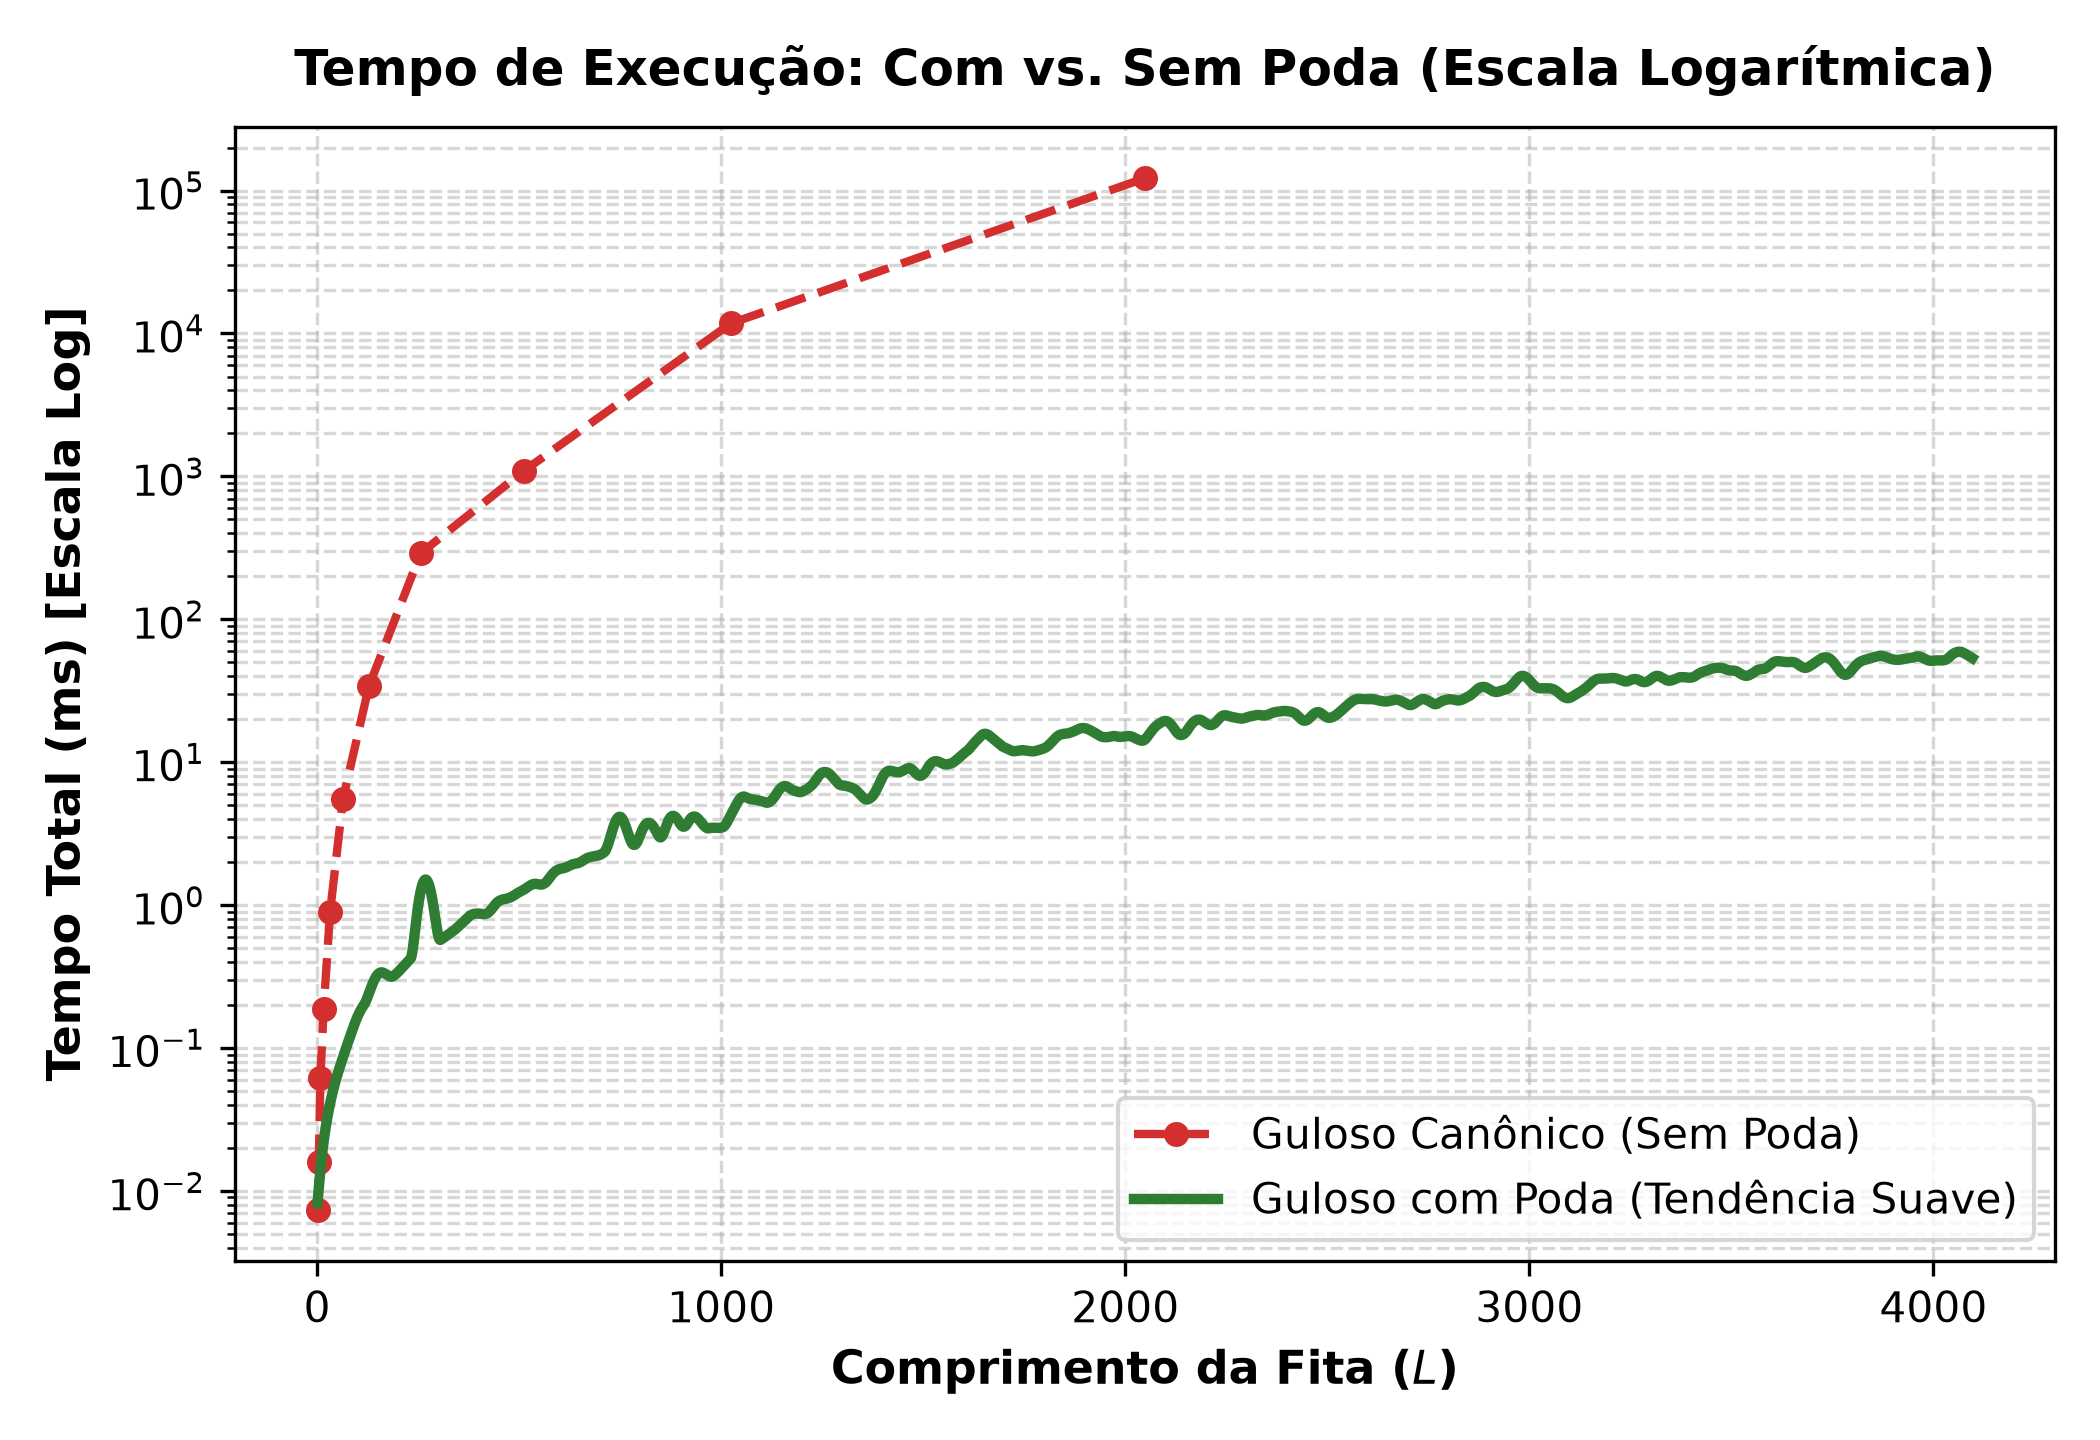
\includegraphics[width=\columnwidth]{grafico_guloso_comparativo_com_e_sem_poda.png}
\caption{Comparativo empírico de tempo na Busca Gulosa com e sem poda de ciclos.}
\label{fig:guloso_poda}
\end{figure}

\subsection{Análise de Desempenho e Escalabilidade (\texorpdfstring{$L = 2$ a $4096$}{L=2 a 4096})}

O número de intervalos contíguos $[i, j]$ para uma fita de tamanho $L$ define o fator de ramificação exato da árvore de busca, dado pela soma das $L$ inversões unitárias com as combinações de blocos: $b(L) = L(L+1)/2 = \Theta(L^2)$. Para a fita de $L = 23$, cada nó gera $b = 276$ sucessores, governando a complexidade espacial do BFS em $O(b^d)$.

\paragraph{Metodologia de Pior Caso por Faixa de Bits.}
Para avaliar o limite superior (\textit{upper bound}) de consumo de recursos e determinar o tamanho máximo das árvores geradas em cada faixa de bits, os experimentos basearam-se no \textbf{pior caso teórico}: fitas com bits alternados (\texttt{'010101...'}). Essa configuração maximiza os blocos unitários e empurra a profundidade para o diâmetro máximo do grafo, $d_{\max} = \lceil L/2 \rceil$.

Sob esse estresse máximo, a quantidade de nós expandidos explode exponencialmente (Figura~\ref{fig:bfs_nos}): enquanto para $L=4$ o BFS expande $1{,}5$ nós e para $L=10$ são $153$ nós ($0{,}54\text{ ms}$), em $L=16$ expandem-se $13.512$ nós e para $L=20$ são necessários $263.922$ nós ($2{,}96\text{ s}$). Para $L > 20$, o pior caso exige varrer quase todo o espaço de estados ($2^{23} \approx 8{,}38 \times 10^6$ nós para $L=23$), esgotando a memória RAM disponível. Os gráficos das Figuras~\ref{fig:bfs_nos} e \ref{fig:guloso_poda} têm como base essa análise limite.

\paragraph{Validação na Fita Oficial e Limite \texorpdfstring{$L = 4096$}{L=4096}.}
Em contrapartida, na fita canônica de $23$ bits proposta pelo docente, os 1s agrupam-se em apenas 5 blocos, permitindo ao BFS encontrar o ótimo em profundidade $d = 5$ ($752.059$ nós e $35{,}42\text{ s}$). Já o Guloso com poda de ciclos, além de resolver a fita oficial em $0{,}16\text{ ms}$, manteve tempo de execução sub-segundo até $L = 4096$ (Tabela~\ref{tab:bench}): mesmo sob fator de ramificação $b(4096) \approx 8{,}39 \times 10^6$ sucessores por nó, convergiu em apenas $48{,}56\text{ ms}$.

\begin{table}[htbp]
\centering
\caption{Desempenho da Busca Gulosa com Poda ($h_2$) até $L = 4096$.}
\label{tab:bench}
\resizebox{\columnwidth}{!}{%
\begin{tabular}{rrrrr}
\toprule
$L$ & Fator $b(L)$ & Custo Médio & Nós Expandidos & Tempo (ms) \\
\midrule
4 & 10 & 1,0 & 1,0 & 0,003 \\
16 & 136 & 4,0 & 4,0 & 0,023 \\
64 & 2.080 & 5,0 & 5,0 & 0,097 \\
256 & 32.896 & 10,0 & 10,0 & 1,189 \\
1024 & 524.800 & 12,0 & 12,0 & 4,643 \\
4096 & 8.390.656 & 12,0 & 12,0 & 48,563 \\
\bottomrule
\end{tabular}%
}
\end{table}

\section{Parte II: Otimização Contínua com Gradiente Descendente}

\subsection{Mapeamento Fuzzy e Espaço de Soluções}

Mapear a sequência de bits para um escalar inteiro $N \in \mathbb{N}$ geraria descontinuidades severas na reta real: inverter o bit mais significativo produziria saltos de amplitude $2^{L-1}$, induzindo falsas divergências no gradiente.

Pelo relaxamento \textit{fuzzy}, o $k$-ésimo bit da fita torna-se uma variável contínua independente:
\begin{equation}
x_k \in [0, 1], \quad \forall k \in \{1, 2, \dots, L\}
\end{equation}
A fita passa a descrever um vetor $\mathbf{x} \in \mathbb{R}^L$ em um hipercubo unitário, onde o alvo nulo corresponde à origem $\mathbf{y} = \mathbf{0}$. O objetivo consiste em encontrar uma trajetória contínua que altere $x_k$ penalizando alterações não-consecutivas.

\subsection{Função Erro \texorpdfstring{$\mathcal{L}(\mathbf{x})$}{L(x)} e Relação com as Transformações}

A função de erro quadrático é definida por:
\begin{equation}
\mathcal{L}(\mathbf{x}) = \sum_{k=1}^L (x_k - y_k)^2
\end{equation}
Para o alvo nulo $\mathbf{y} = \mathbf{0}$, $\mathcal{L}(\mathbf{x}) = \sum_{k=1}^L x_k^2$. Nos vértices booleanos $\{0, 1\}^L$, $\mathcal{L}(\mathbf{x})$ coincide exatamente com a Distância de Hamming $h_1(\mathbf{x})$. Minimizar $\mathcal{L}(\mathbf{x})$ atrai continuamente cada coordenada para zero, e o vetor deslocamento entre iterações consecutivas $\Delta \mathbf{x}^{(t)} = \mathbf{x}^{(t+1)} - \mathbf{x}^{(t)} = -\eta \nabla \mathcal{L}(\mathbf{x}^{(t)})$ representa a transformação contínua instantânea aplicada à fita.

\subsection{Gradiente Descendente sem Custo e Comportamento de \texorpdfstring{$\eta$}{eta}}

A regra clássica de atualização é dada por:
\begin{equation}
x_i \leftarrow x_i - \eta \frac{\partial \mathcal{L}}{\partial x_i} = x_i - 2\eta (x_i - y_i)
\end{equation}
Para $y_i = 0$, a dinâmica analítica desacoplada é:
\begin{equation}
x_i^{(t+1)} = (1 - 2\eta) x_i^{(t)}
\end{equation}
Essa recorrência expressa formalmente três regimes de operação:
\begin{itemize}[nosep]
    \item \textbf{Subcrítico ($\eta < 0{,}5$):} O fator de contração permanece positivo e menor que $1$ (por exemplo, $0{,}8$ para $\eta = 0{,}1$), produzindo decaimento exponencial suave e monótono em direção ao estado nulo.
    \item \textbf{Crítico Unitário ($\eta = 0{,}5$):} O fator anula-se identicamente, zerando todo o resíduo da função erro em \textbf{um único passo exato}.
    \item \textbf{Violação de Domínio e Divergência ($\eta > 0{,}5$):} O passo ultrapassa o mínimo global e projeta o bit para valores negativos (atingindo $-0{,}5$ para $\eta = 0{,}75$), violando o domínio fuzzy $[0, 1]$. Para $\eta = 1{,}0$, o bit oscila perpetuamente entre $+1$ e $-1$ sem convergir, e para $\eta > 1{,}0$, o erro diverge de forma ilimitada.
\end{itemize}

\paragraph{Sequência de Transformações.}
Os vetores diferença entre passos consecutivos $\Delta \mathbf{x}^{(t)} = \mathbf{x}^{(t+1)} - \mathbf{x}^{(t)}$ representam a sequência de transformações do algoritmo contínuo. Para $\eta = 0{,}5$, a convergência ocorre em 1 único passo exato com o vetor $\Delta \mathbf{x}^{(0)} = -\mathbf{x}_0$, aplicando $-1$ pontualmente nas nove posições ativas. Para $\eta = 0{,}1$, obtém-se uma sequência de transformações amortecidas que acumulam assintoticamente o cancelamento total do vetor inicial.

A Figura~\ref{fig:topografia_etas} ilustra as curvas de nível da perda quadrática e as trajetórias geradas para cada regime de $\eta$, evidenciando a convergência imediata para $\eta = 0{,}5$, a oscilação com valores negativos para $\eta = 0{,}75$ e a divergência explosiva para $\eta = 1{,}05$.

\begin{figure}[htbp]
\centering
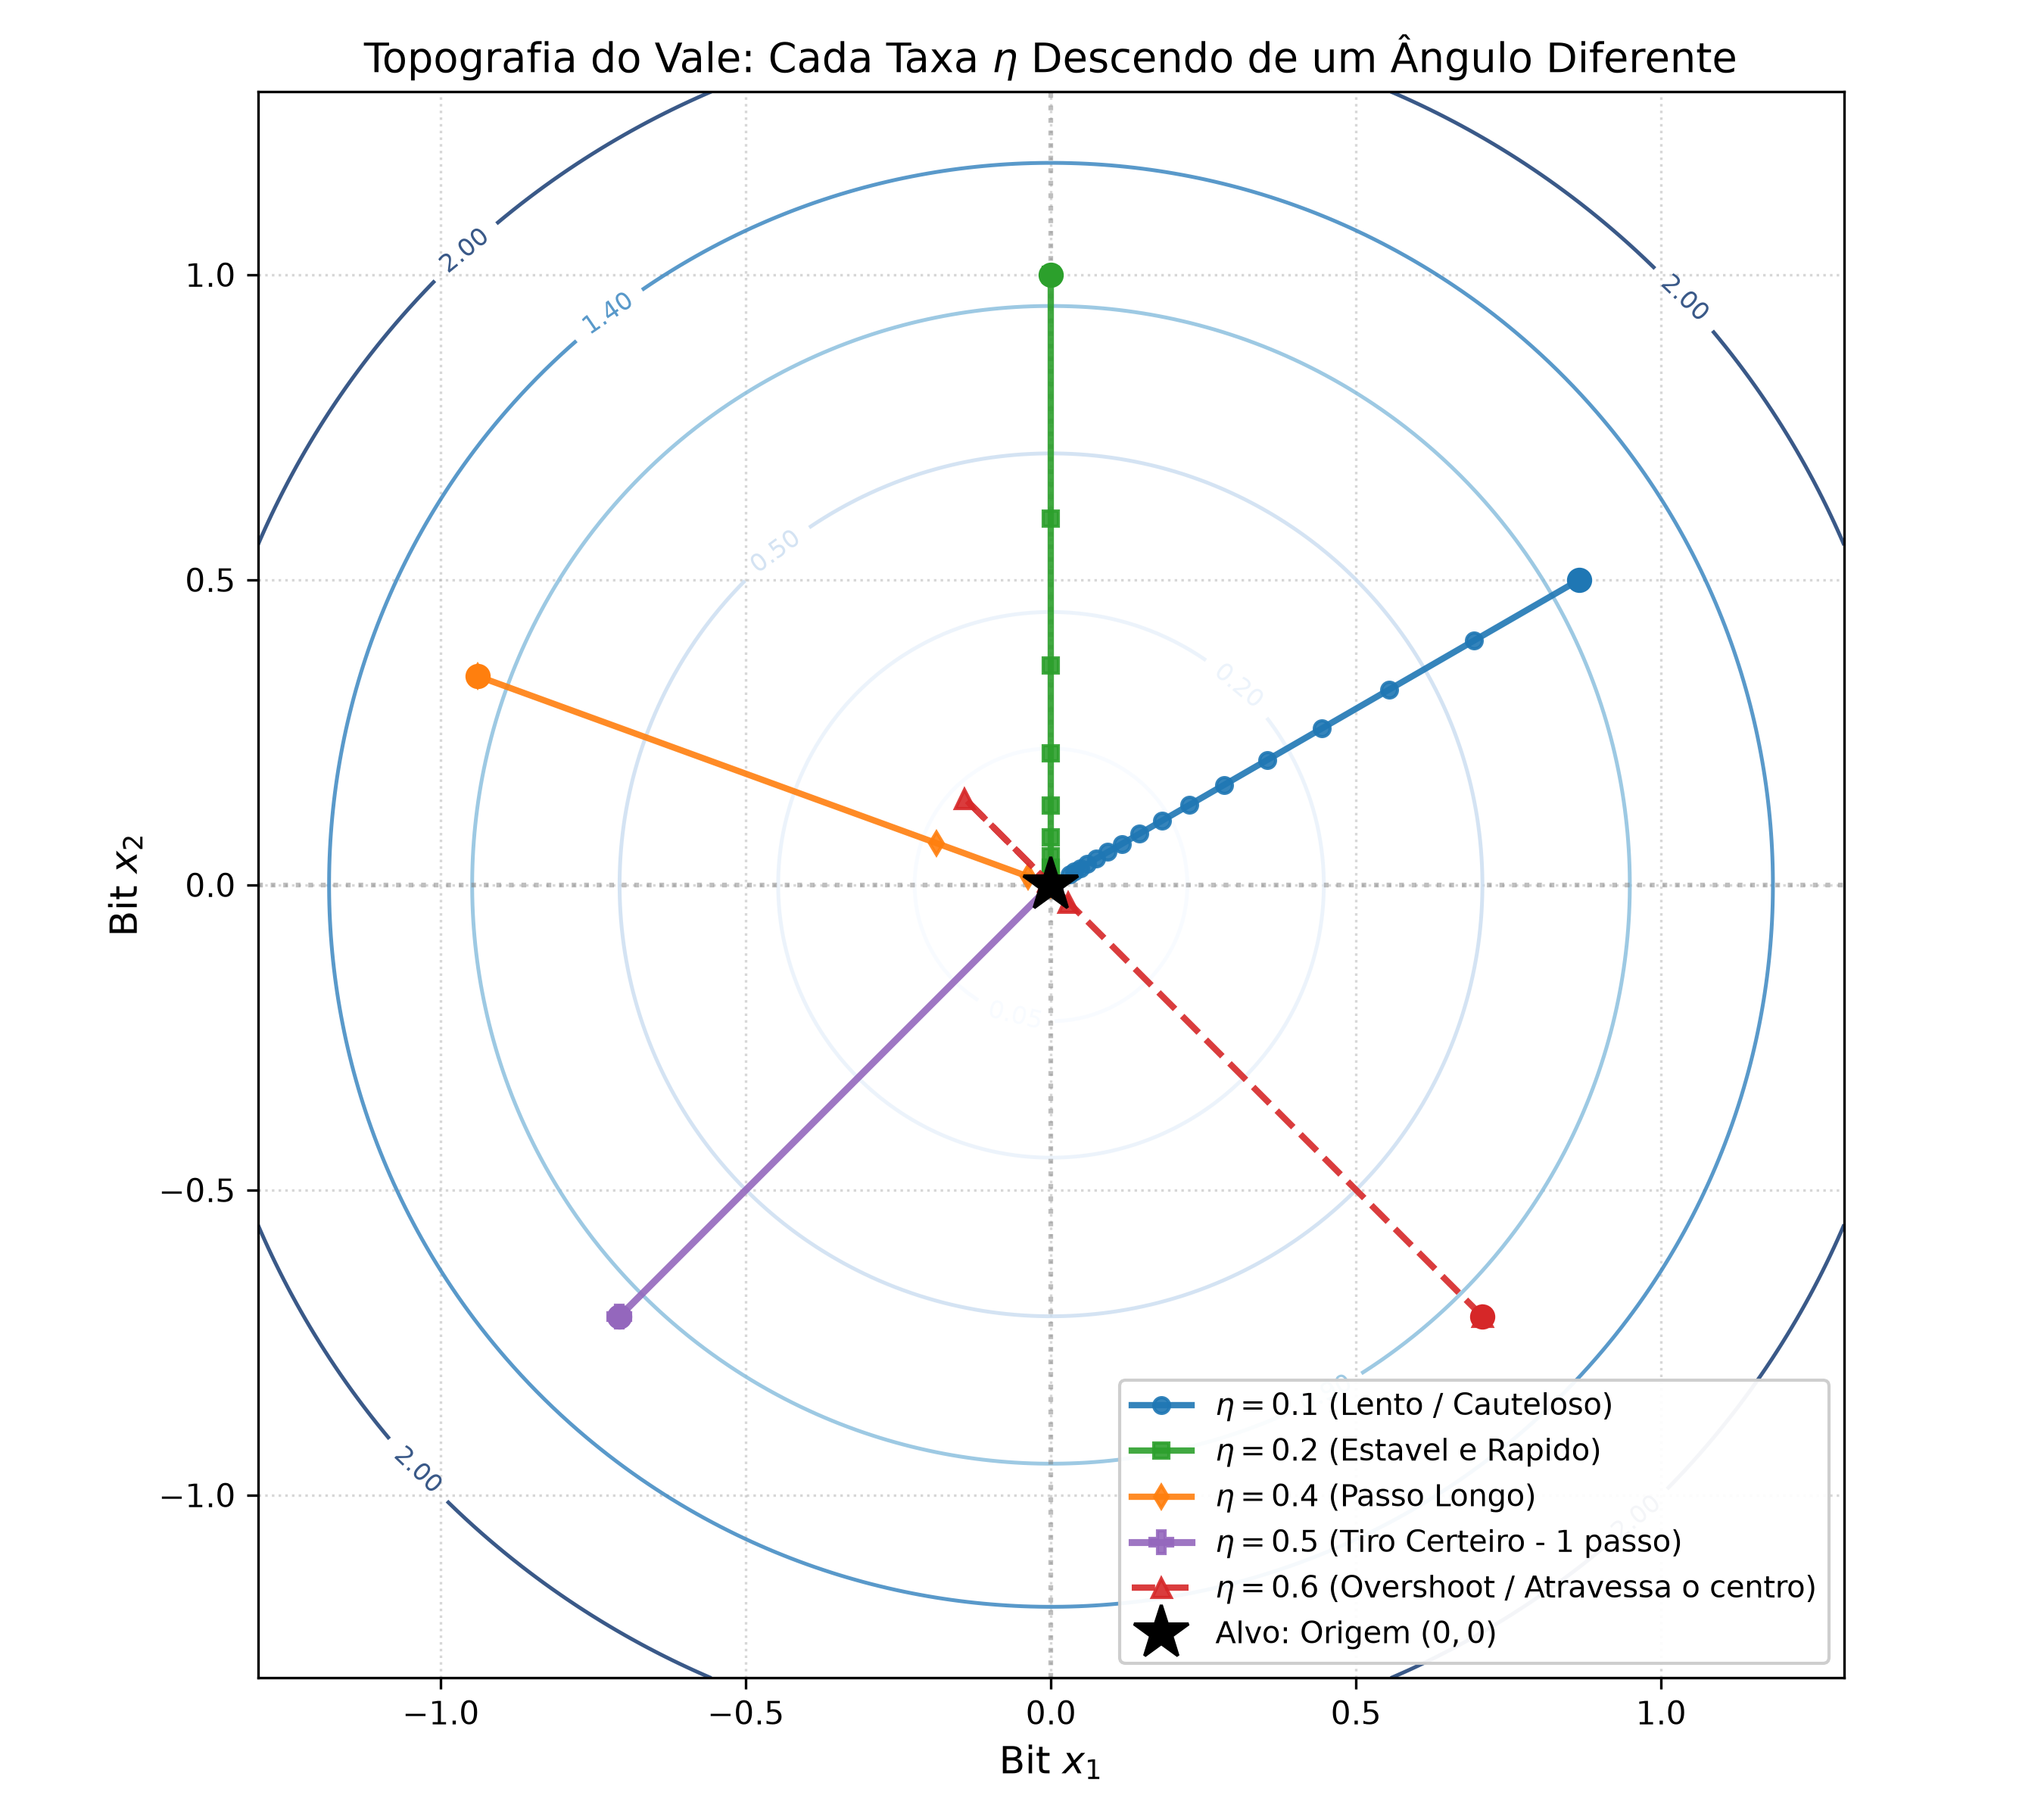
\includegraphics[width=0.85\columnwidth]{01_topografia_curvas_nivel_etas_direcoes.png}
\caption{Curvas de nível de $\mathcal{L}(\mathbf{x})$ e trajetórias 2D do Gradiente Descendente para múltiplos valores de $\eta$.}
\label{fig:topografia_etas}
\end{figure}

\subsection{Inclusão da Função Custo \texorpdfstring{$C(z)$}{C(z)} e Regra da Cadeia}

Para favorecer inversões adjacentes e penalizar mutações isoladas, o vetor $z$ modela a intensidade da transformação através do gradiente: $z_i = |\nabla_i \mathcal{L}(\mathbf{x})| = 2|x_i|$ (ou suave $z_i = x_i$). Definimos a função custo contígua via diferença quadrática entre vizinhos adjacentes:
\begin{equation}
C(\mathbf{x}) = \sum_{k=1}^{L-1} (x_{k+1} - x_k)^2
\end{equation}
Essa função anula-se quando coordenadas vizinhas variam em uníssono (blocos uniformes) e atinge valores máximos em alternâncias de alta frequência.

Considerando a perda regularizada $J(\mathbf{x}) = \mathcal{L}(\mathbf{x}) + \lambda C(\mathbf{x})$, aplicamos a regra da cadeia para uma coordenada interna $x_i$ ($1 < i < L$):
\begin{equation}
\begin{split}
\frac{\partial J}{\partial x_i} &= \frac{\partial \mathcal{L}}{\partial x_i} + \lambda \frac{\partial C}{\partial x_i} \\
&= 2x_i + 2\lambda (2x_i - x_{i-1} - x_{i+1})
\end{split}
\end{equation}
\textbf{Demonstração da influência adjacente:} O termo $2\lambda (2x_i - x_{i-1} - x_{i+1})$ evidencia que a taxa de variação de $x_i$ é diretamente governada pelas coordenadas dos vizinhos imediatos $x_{i-1}$ e $x_{i+1}$.

\subsection{Minimização para Diferentes Valores de \texorpdfstring{$\lambda$}{lambda} e Limite de Estabilidade}

A equação do gradiente revela comportamentos distintos conforme a configuração local de vizinhança:
\begin{itemize}[nosep]
    \item \textbf{Interior do Bloco ($1, 1, 1$):} A simetria entre as coordenadas adjacentes anula a penalidade de regularização, conduzindo a atualização unicamente pelo gradiente da função erro ($2x_i$).
    \item \textbf{Borda do Bloco ($0, 1, 1$):} A descontinuidade lateral gera uma força de atração proporcional a $2\lambda$, retardando a modificação prematura da extremidade.
    \item \textbf{Bit Isolado ($0, 1, 0$):} Com vizinhos nulos, a penalidade atinge intensidade máxima e amplifica o gradiente efetivo para $2x_i + 4\lambda$. Esse ganho acelera a eliminação do bit solitário como ruído de alta frequência antes da remoção dos blocos contíguos.
\end{itemize}

\paragraph{Cota Crítica de Estabilidade.} A derivada segunda de $J$ em relação a cada coordenada é $\frac{\partial^2 J}{\partial x_i^2} = 2 + 4\lambda$. Valores elevados de $\lambda$ aumentam a curvatura da função de custo. Para evitar oscilações divergentes, a taxa de aprendizado deve respeitar o limite:
\begin{equation}
\eta \le \eta_{\mathrm{crit}} \approx \frac{1}{2 + 4\lambda}
\end{equation}
Caso $\eta$ ultrapasse essa cota, as atualizações consecutivas amplificam o erro em vez de reduzi-lo, resultando em divergência numérica ($J \to \infty$). Para $\lambda = 20{,}0$, a restrição impõe $\eta \le 0{,}0122$. O diagrama de fase empírico confrontado com a curva teórica é apresentado na Figura~\ref{fig:diagrama_fase}.

\begin{figure}[htbp]
\centering
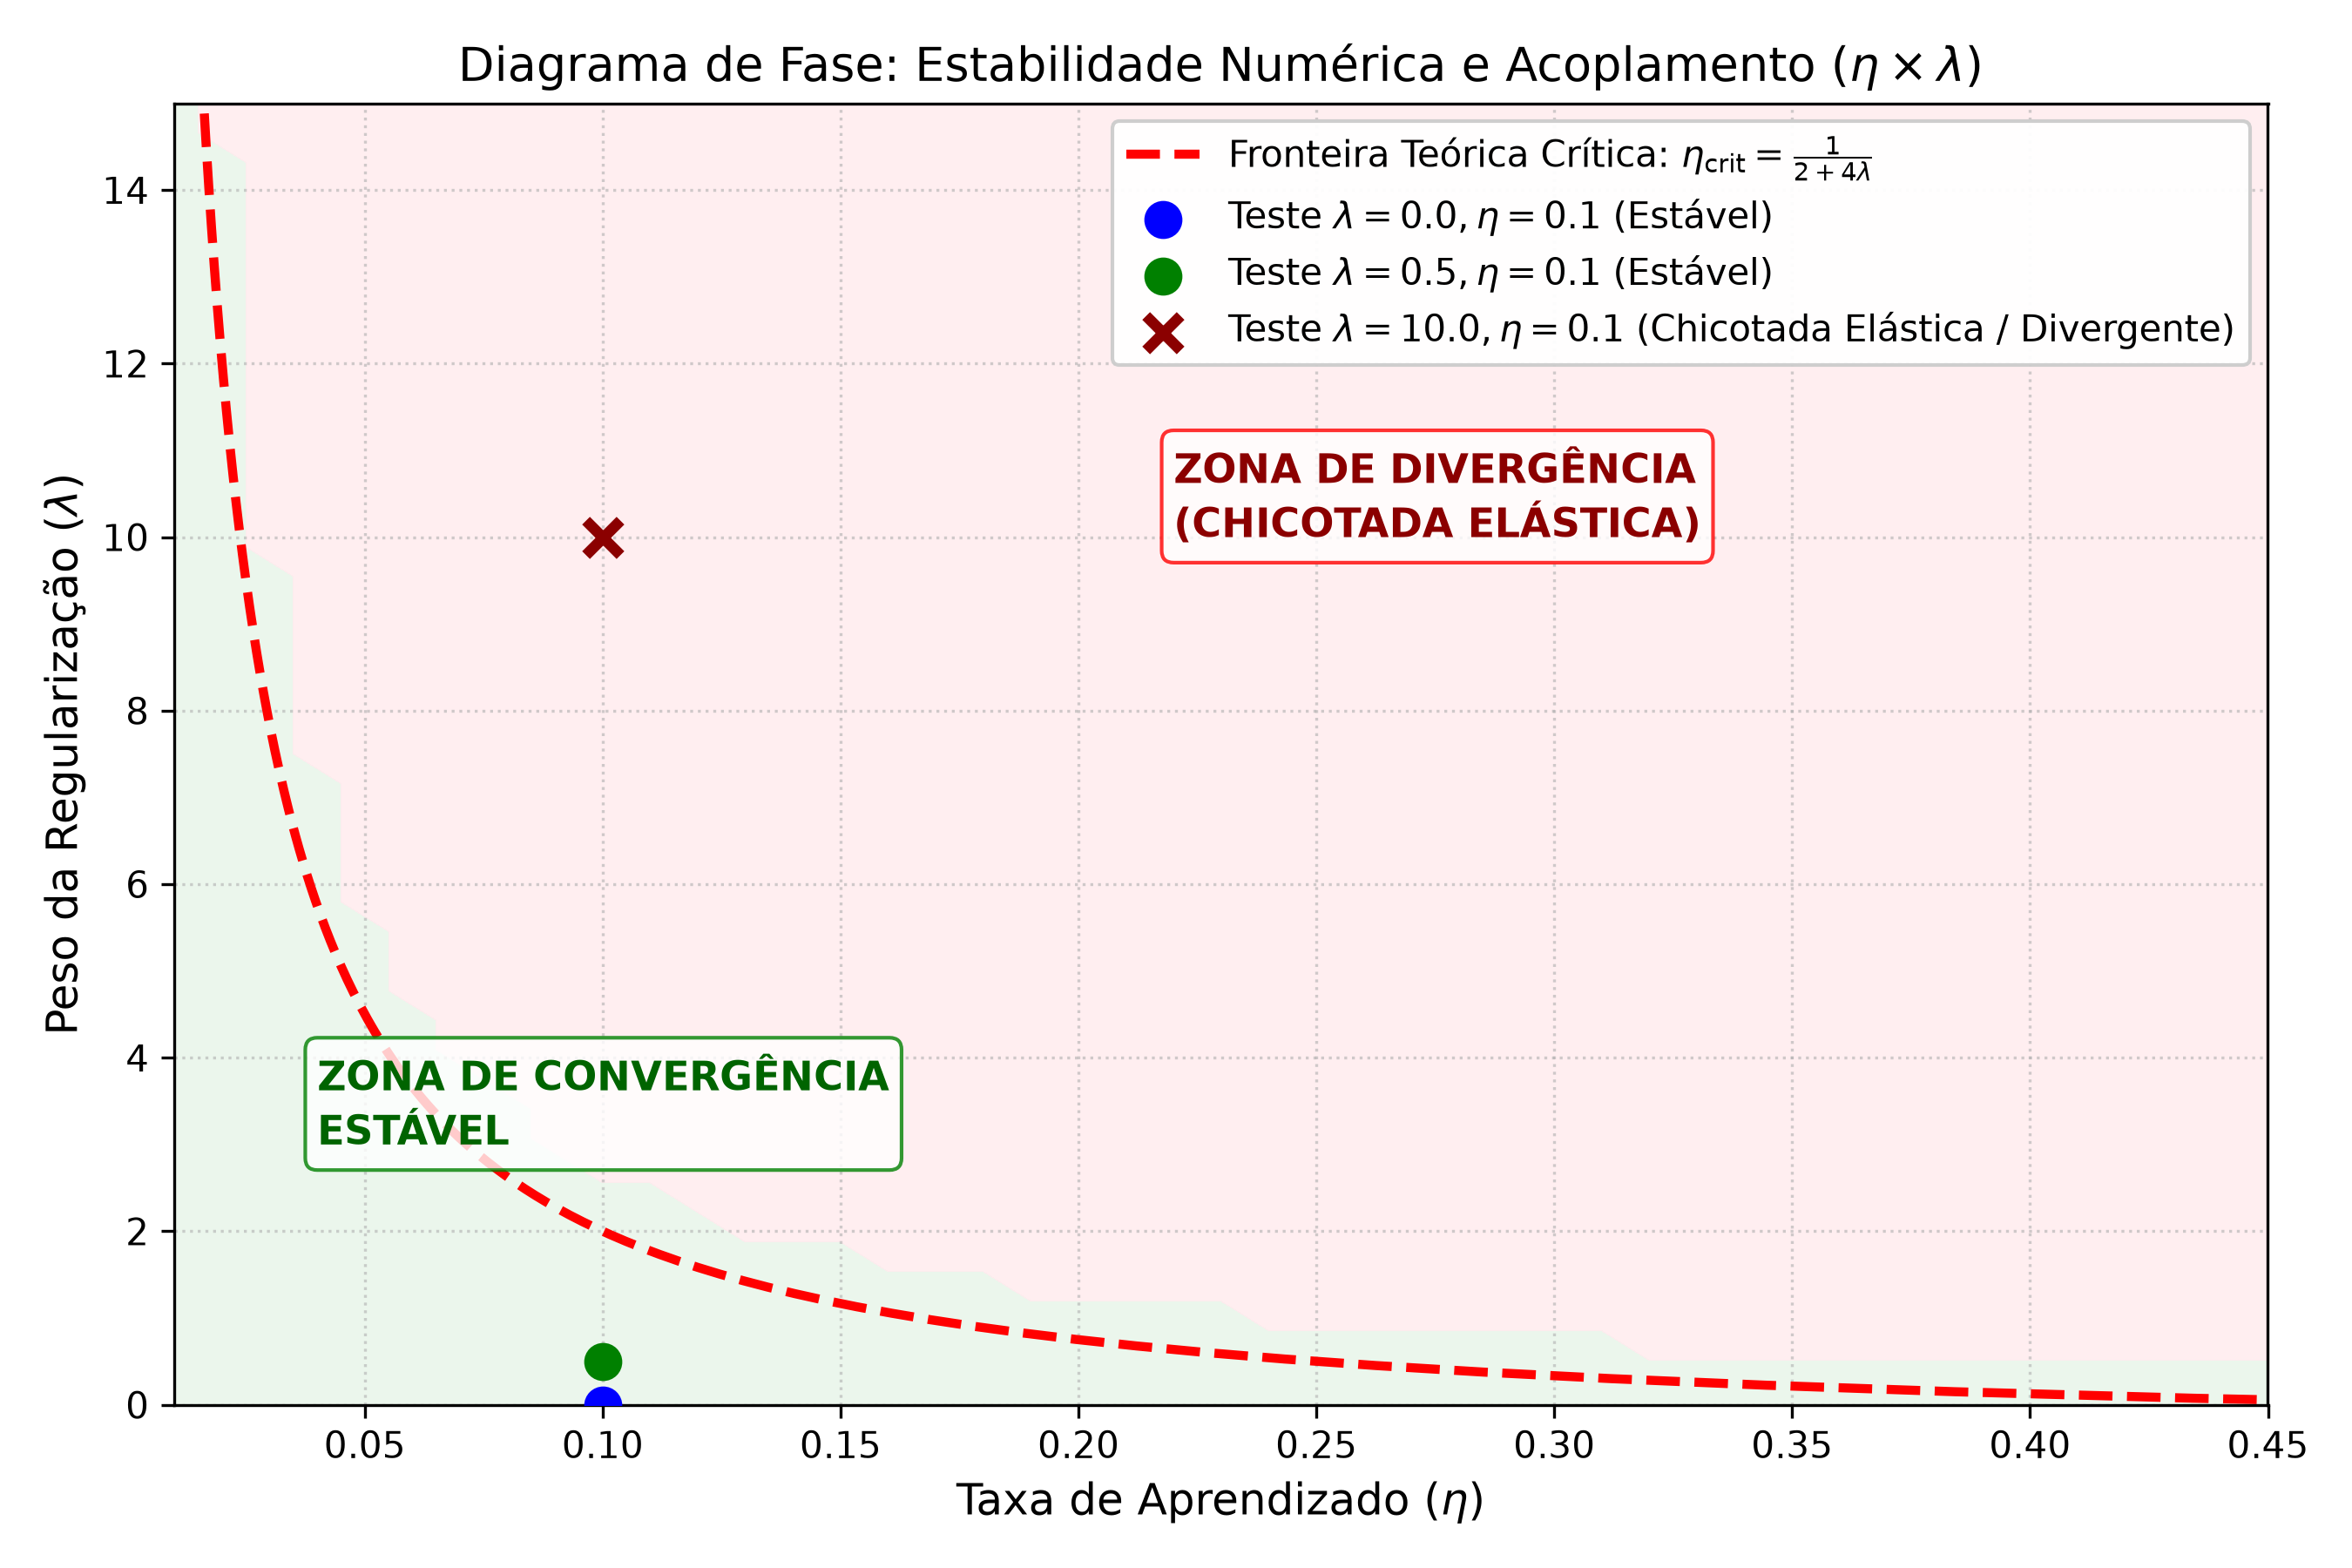
\includegraphics[width=0.75\columnwidth]{06_diagrama_fase_estabilidade_eta_lambda.png}
\caption{Diagrama de fase de estabilidade numérica no plano $(\eta, \lambda)$ e curva limite teórica de estabilidade.}
\label{fig:diagrama_fase}
\end{figure}

\section{Considerações Finais}

A formulação do trabalho demonstra a dualidade entre espaços de busca em IA: no domínio discreto, o BFS garante a solução de custo mínimo 5 e o algoritmo Guloso com poda de ciclos viabiliza a execução escalável até $L = 4096$; no domínio contínuo, o relaxamento fuzzy com gradiente descendente atinge o alvo em passo único para $\eta = 0{,}5$, enquanto a função custo contígua preserva a inversão em bloco respeitando a cota de estabilidade $\eta \le \frac{1}{2 + 4\lambda}$.

\begin{thebibliography}{00}
\footnotesize
\setlength{\itemsep}{0pt}
\setlength{\parskip}{0pt}
\bibitem{russell2020}
RUSSELL, S.; NORVIG, P. \textbf{Artificial Intelligence: A Modern Approach}. 4. ed. Pearson, 2020. Cap. 3: Solving Problems by Searching.

\bibitem{smola2023}
SMOLA, A. et al. \textbf{Dive into Deep Learning}. Cambridge University Press, 2023. Cap. 12: Optimization Algorithms.

\bibitem{paszke2019}
PASZKE, A. et al. PyTorch: An Imperative Style, High-Performance Deep Learning Library. \textbf{NeurIPS 32}, p. 8024--8035, 2019.
\end{thebibliography}

\end{document}
